\documentclass{beamer}
\usepackage{graphicx}
\usepackage{amsmath, amsthm, amsfonts, amssymb, mathrsfs, mathtools}
\usepackage{textcomp} % straigth apos
\usepackage{tikz}
\usepackage{verbatim}
\usepackage{tikzit}
\usepackage{listings}
\usepackage{subfig}
\usepackage[ruled,vlined, linesnumbered]{algorithm2e}
\usepackage{algorithmic,float}
\usepackage[
  audience=short
  % audience=long
]{beameraudience}

\input{graphs.tikzstyles}
\usetikzlibrary{decorations.pathreplacing}

\usefonttheme{serif}

\theoremstyle{definition}

\setbeamercovered{invisible}

\setbeamertemplate{theorems}[numbered]
\setbeamertemplate{lemma}[numbered]
\newtheorem{remark}{Remark}

\newcommand{\xra}[1]{\overset{#1}{\rightsquigarrow}}
\newcommand{\verysmall}{\scriptsize}
\newcommand{\vect}[2]{%
\begin{bmatrix}
    #1 \\
    #2
\end{bmatrix}
}


\usetheme{Madrid}
\useoutertheme{tree} % Alternatively: miniframes, infolines, split
\useinnertheme{circles}


\setbeamertemplate{headline}
{%
  \leavevmode%
  \begin{beamercolorbox}[wd=.5\paperwidth,ht=2.5ex,dp=1.125ex]{section in head/foot}%
    \hbox to .5\paperwidth{\hfil\insertsectionhead\hfil}
  \end{beamercolorbox}%
  \begin{beamercolorbox}[wd=.5\paperwidth,ht=2.5ex,dp=1.125ex]{subsection in head/foot}%
    \hbox to .5\paperwidth{\hfil\insertsubsectionhead\hfil}
  \end{beamercolorbox}%
}

\setbeamertemplate{section in toc}{%
  \inserttocsectionnumber.~\inserttocsection}
\setbeamercolor{section in toc}{fg=black}
\setbeamercolor{subsection in toc}{fg=structure}
\setbeamertemplate{subsection in toc}{%
  \hspace{1.2em}{\tiny\inserttocsectionnumber.\inserttocsubsectionnumber}~\small\inserttocsubsection\par}

% \setbeamertemplate{bibliography item}{\insertbiblabel.~\insertbibitem}

\definecolor{lightbrown}{RGB}{207, 161, 118}

\usecolortheme[named=lightbrown]{structure}

\title[Model Checking Real-Time Systems]{Model Checking Real-Time Systems}
\date{December 12, 2022}
\author[V. Trélat]{Vincent Trélat}
\institute[TUM]{Technical University of Munich}

\begin{document}

\begin{frame}
\titlepage
\end{frame}

\begin{frame}
\tableofcontents
\end{frame}

\section{Timed Automata}
\subsection{Preliminaries}

\begin{frame}
  Set of \emph{time values}: $\mathbb{R}_{\geq 0}$
  \vfill
  \emph{Timed words} over $\Sigma \times \mathbb{R}_{\geq 0}$
  \vfill
  Set of \emph{valuations} over a set of clocks $C$: $\mathbb{R}_{\geq 0}^C$
  \vfill
  \emph{Constraints} over $C$: $\varphi ::= x \odot k\ |\ \varphi \land \varphi$ where $x \in C$, $k \in \mathbb{Z}$ and $\odot \in \{<, \leq, =, \geq, >\}$
  \vfill
  Set of valuations \emph{satisfying} $\varphi$: $[\![\varphi]\!]_C = \{v \in \mathbb{R}_{\geq 0}^C\ |\ v \models \varphi\}$
\end{frame}


\subsection{Timed Automata}

\begin{frame}
  \begin{definition}
    A \emph{Timed Automaton} (TA) $\mathcal{A}$ is the tuple $(L, \ell_0, C, \Sigma, I, E)$ where:
    \begin{itemize}
      \item $L$ is a finite set of \emph{locations} with initial location $\ell_0 \in L$
      \item $C$ is a finite set of \emph{clocks}
      \item $\Sigma$ is a finite set of \emph{actions}
      \item $I \colon L \to \varPhi(C)$ is an \emph{invariant mapping}
      \item $E \subseteq L \times \varPhi(C) \times \Sigma \times 2^{C} \times L$ is a set of edges
      \item a set $F$ of \emph{target locations} is generally specified
    \end{itemize}
  \end{definition}
  \vfill
  Edges are denoted by $\ell \xrightarrow{\varphi, a, r} \ell'$.
\end{frame}
\begin{frame}
  Example of a TA with 3 locations, 2 clocks and 2 actions (letters):
  \ctikzfig{ex_ta}
\end{frame}

\begin{frame}{Operational Semantics}
\onslide<1->{
\begin{figure}
  \centering
  \begin{tikzpicture}
  \small
	\begin{pgfonlayer}{nodelayer}
		\node [style=white, align=center] (0) at (-2, 0) {$\ell$ \\ $y \leq 1$};
		\node [style=white, align=center] (1) at (2, 0) {$\ell'$ \\ $y \leq 2$};
		\node [style=none] (2) at (0, -0.25) {$x > 1, x := 0$};
		\node [style=none] (3) at (0, 0.25) {$a$};
	\end{pgfonlayer}
	\begin{pgfonlayer}{edgelayer}
		\draw [->, thick] (0) -- (1);
	\end{pgfonlayer}
\end{tikzpicture}
\end{figure}
}
\onslide<2->{
  \begin{equation*}
    \begin{cases}
      v(x) = {\color{red}3.4}\\
      v(y) = {\color{red}0.9}
    \end{cases}
    \onslide<3->{
    \quad
    (\ell, v) \xrightarrow{\ \ a\ \ } (\ell', v')
    \quad
    }
    \onslide<4->{
    \begin{cases}
      v'(x) = {\color{red}0}\\
      v'(y) = {\color{red}0.9}
    \end{cases}
    }
  \end{equation*}
}
\onslide<5->{
  \begin{equation*}
    \begin{cases}
      v(x) = {\color{red}1.2}\\
      v(y) = {\color{red}0.2}
    \end{cases}
    \onslide<6->{
    \quad
    (\ell, v) \xrightarrow{{\color{red}0.5},\ a} (\ell', v')
    \quad
    }
    \onslide<7->{
    \begin{cases}
      v'(x) = {\color{red}0}\\
      v'(y) = {\color{red}0.7}
    \end{cases}
    }
  \end{equation*}
}
\end{frame}

\begin{frame}{Operational Semantics}
  \only<1>{
  \begin{figure}
    \centering
    \begin{tikzpicture}
    \small
    \begin{pgfonlayer}{nodelayer}
      \node [style=white, align=center] (0) at (-2, 0) {$\ell$ \\ $y \leq 1$};
      \node [style=white, align=center] (1) at (2, 0) {$\ell'$ \\ $y \leq 2$};
      \node [style=none] (2) at (0, -0.25) {$x > 1, x := 0$};
      \node [style=none] (3) at (0, 0.25) {$a$};
    \end{pgfonlayer}
    \begin{pgfonlayer}{edgelayer}
      \draw [->, thick] (0) -- (1);
    \end{pgfonlayer}
  \end{tikzpicture}
  \end{figure}
  }
  \only<2->{
  \begin{figure}
    \centering
    \begin{tikzpicture}
    \small
    \begin{pgfonlayer}{nodelayer}
      \node [style=white, align=center] (0) at (-2, 0) {$\ell$ \\ $\ I(\ell)\ $};
      \node [style=white, align=center] (1) at (2, 0) {$\ell'$ \\ $\ I(\ell')\ $};
      \node [style=none] (2) at (0, -0.25) {$\varphi, r$};
      \node [style=none] (3) at (0, 0.25) {$a$};
    \end{pgfonlayer}
    \begin{pgfonlayer}{edgelayer}
      \draw [->, thick] (0) -- (1);
    \end{pgfonlayer}
  \end{tikzpicture}
  \end{figure}
  }
  \only<3>{
  \begin{equation*}
    (\ell, v) \xrightarrow{d,\ a} (\ell', v')
  \end{equation*}
  }
  \only<4->{
  \begin{equation*}
    (\ell, v) \xrightarrow{d,\ a} (\ell', (v+d)[r])
  \end{equation*}
  }
  \onslide<5->{
  provided that:
  $$\ell \xrightarrow{\varphi, a, r} \ell'\ \text{is a transition in the TA}$$
  $$\forall t \in [0, d], \ v + t \models I(\ell)$$
  $$(v + d)[r] \models I(\ell')$$
  }
\end{frame}

\justfor{long}{
\begin{frame}
  \frametitle{Operational Semantics}
\begin{definition}
  \small
  The \emph{operational semantics} of a TA $A = (L, \ell_0, C, \Sigma, I, E)$ is the infinite-state timed transition system $[\![A]\!] = (S, s_0, \Sigma \times \mathbb{R}_{\geq 0}, T)$, where
  \begin{align*}
	  &S := \{(\ell, v) \in L \times \mathbb{R}_{\geq 0}^C\ |\ v \models I(\ell)\}, \quad s_0 := (\ell_0, \text{\bf 0}_C),\\
	  &T := \{(\ell, v) \xrightarrow{d, a} (\ell', (v+d)[r]) \ | \ d \in \mathbb{R}_{\geq 0}, \\
    &\quad\quad\quad\quad\forall d' \in [0, d], v + d' \models I(\ell) \land \exists \ell \xrightarrow{\varphi, a, r} \ell' \in E, v + d \models \varphi \}
  \end{align*}
\end{definition}
\end{frame}
}

\begin{frame}
  \small
  \ctikzfig{ex_ta}
  $$ \left(\ell_0, \vect{0.6}{1}\right) \xrightarrow{0.4, a} \left(\ell_1, \vect{1}{0}\right) \xrightarrow{1,b} \left(\ell_2, \vect{2}{1}\right) \xrightarrow{0.6, a} \left(\ell_0, \vect{0}{1.6}\right) \xrightarrow{0, b} \left(\ell_0, \vect{0}{0}\right)$$
\end{frame}

\subsection{Regions and zones}

\begin{frame}
  \tableofcontents[currentsection, currentsubsection]
\end{frame}

\begin{frame}
  \onslide<1->{
    \begin{center}
      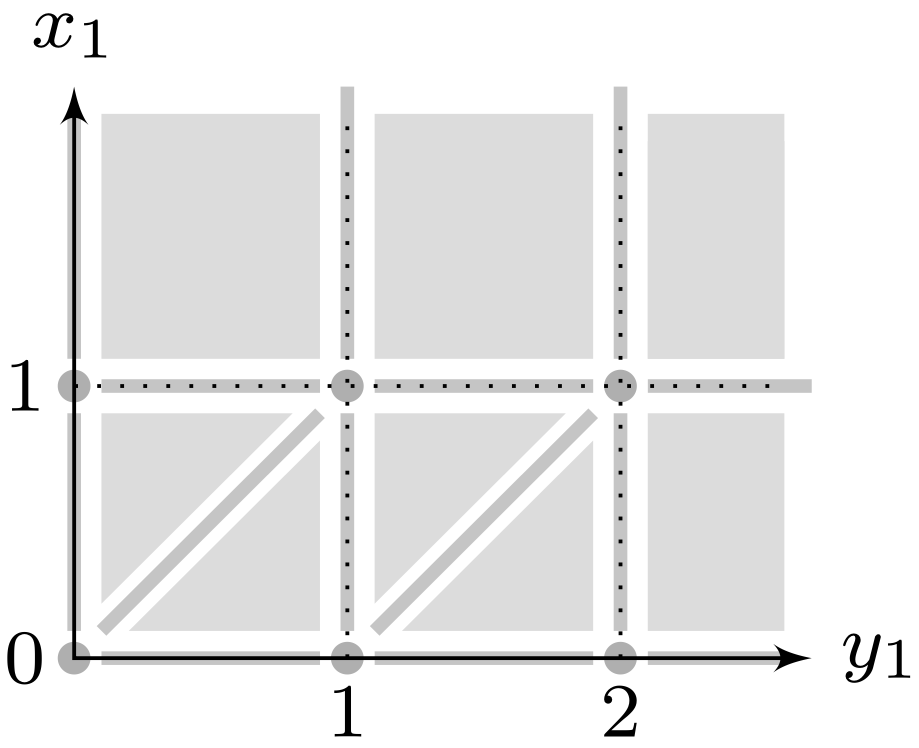
\includegraphics[height=8.4em]{../img/TAreg.png}
    \end{center}
  }
  \onslide<2->{
  \begin{definition}
  \small
  Two valuations $v, v' \in \mathbb{R}_{\geq 0}^C$ are region equivalent, i.e\ $v \cong_M v'$ iff:
  \begin{itemize}
    \item<3-> $\forall x \in C, \lfloor v(x) \rfloor = \lfloor v'(x) \rfloor \ \lor \ v(x), v'(x) > M_x$\\
    {\verysmall\color{blue}their integral parts on any clock are equal}
    \item<4-> $\forall x \in C, \langle v(x) \rangle = 0 \Leftrightarrow \langle v'(x) \rangle = 0 \ \lor \ v(x) \geq M_x$\\
    {\verysmall\color{blue}their fractional parts on any clock are simultaneously equal to zero}
    \item<5-> $\forall x, y \in C, \langle v(x) \rangle \leq \langle v(y) \rangle \Leftrightarrow \langle v'(x) \rangle \leq \langle v'(y) \rangle \ \lor \ v(x) > M_x \ \lor \ v(y) > M_y$\\
    {\verysmall\color{blue}the order of their fractional parts on any two clocks is preserved}
  \end{itemize}
\end{definition}
  }
\end{frame}

\begin{frame}
\begin{definition}[Region Automaton]
  $\mathcal{R}_{\cong_M}(A) = (S, s_0, \Sigma, T)$ is the \emph{region automaton} of $A$, where:
  \begin{itemize}
    \item $S := (L \times \mathbb{R}_{\geq 0}^C)_{/\cong_M},\ s_0 := [\ell_0, \text{\bf 0}_C]_{/\cong_M}$
    \item $T := \{[\ell, v]_{\cong_M} \xrightarrow{a} [\ell', v']_{\cong_M}\ |\ \exists d \in \mathbb{R}_{\geq 0}, (\ell, v) \xrightarrow{d, a} (\ell', v')\}$
  \end{itemize}
\end{definition}
\begin{itemize}
  \item<2> $\left| S \right|$ is exponential in the number of clocks and in the maximal constants of the timed automaton
  \item<2> Is there a way to reduce the number of states?
\end{itemize}
\end{frame}

\begin{frame}
  \small
  Zone: a set of valuations satisfying a constraint over $C$, e.g.\ $[\![\varphi]\!]_C$.
  \begin{center}
    \begin{tikzpicture}
      \node [style=white, align=center] (0) at (-2, 0) {$\ell$\\$I(\ell)$};
      \node [style=white, align=center] (1) at (2, 1) {$\ell'$\\$I(\ell')$};
      \draw [->] (0) to [in=-180, out=0] node [midway, below=4pt, rotate=33] {$\varphi, a, r$} (1);
      \draw [->] (0) to [in=-160, out=160, loop] (0);
      \only<2>{\draw [->, very thick, color=green!80!black] (0) to [in=-160, out=160, loop] (0);}
      \only<3>{\draw [->, very thick, color=green!80!black] (0) to [in=-180, out=0] (1);}
    \end{tikzpicture}
  \end{center}
  \begin{itemize}
    \item<2-> Wait in $\ell$ for a delay $d$ to elapse
    \begin{itemize}
      \item<4-> $Z$ must be ``delayed'' (transition to the upward closure of $Z$)
      \item<4-> $I(\ell)$ must be satisfied over the whole delay
    \end{itemize}
    \item<3-> Take the transition to $\ell'$ (without any delay)
    \begin{itemize}
      \item<5-> $\varphi$ must be satisfied
      \item<5-> $Z$ must be ``reset'' w.r.t.\ $r$
      \item<5-> $I(\ell')$ must be satisfied eventually
    \end{itemize}
  \end{itemize}
  \onslide<6->{
    Need to be normalised!
  }
\end{frame}

\justfor{long}{
\begin{frame}
  \small
  \begin{definition}[Zone]
    A set of valuations $Z \subseteq \mathbb{R}_{\geq 0}^C$ is a zone iff:
    $\exists \varphi \in \varPhi_d(C), Z = [\![\varphi]\!]_C$
    
    In this case, we define:
    \begin{itemize}
      \item the \emph{delay} of $Z$: $Z^\uparrow \triangleq \{ v + d \ |\ v \in Z \land d \in \mathbb{R}_{\geq 0}\}$
      \item the \emph{reset} of $Z$: $Z[r] \triangleq \{ v[r] \ |\ v \in Z\}$ for $r \subseteq C$
    \end{itemize}
  \end{definition}
  \small
  \begin{definition}[Zone automaton]
    The \emph{zone automaton} $[\![A]\!]_Z$ of $A$ is the tuple $(S, s_0, \Sigma \cup \{\delta\}, T)$, where:
    \begin{align*}
      &S := \{ (\ell, Z)\ |\ \ell \in L, Z \in \mathbb{R}_{\geq 0}^C\ \text{is a zone}\},\quad s_0 := (\ell_0, \{\text{\bf 0}_C\})\\
      &T := \{ (\ell, Z) \xra{\delta} (\ell, Z^\uparrow \cap [\![I(\ell)]\!]_C)\} \cup \\
      &\{ (\ell, Z) \xra{a} (\ell', (Z \cap [\![\varphi]\!]_C)[r] \cap [\![I(\ell')]\!]_C) \ |\ \ell \xrightarrow{\varphi, a, r} \ell' \in E\}
    \end{align*}
  \end{definition}
  $\rightarrow$ Normalisation ($\simeq$ quotienting), shortest-path-closed DBM extrapolation
\end{frame}
}

% Remark: if the TA does not contain diagonal constraints, the reachability problem on the TA is equivalent to the reachability problem on the ZA. Otherwise, other normalization techniques are needed.

\justfor{long}{
\begin{frame}
  \centering
  \small
  \begin{tikzpicture}
    \node (sys) at (0, 0) {$
        Z =
        \begin{cases}
          x_1 &\leq 3\\
          x_1 - x_2 &\leq 10\\
          x_1 - x_2 &\geq 4\\
          x_1 - x_3 &\leq 2\\
          x_3 - x_2 &\leq 2\\
          x_3 &\geq -5
        \end{cases}
        $
    };
    \node [draw, circle] (x0) at (4, -1) {$x_0$};
    \node [draw, circle] (x1) at (4, 1) {$x_1$};
    \node [draw, circle] (x2) at (6, 1) {$x_2$};
    \node [draw, circle] (x3) at (6, -1) {$x_3$};
    \draw[->] (x1) -- (x0) node[midway, left] {$3$};
    \draw[->] (x1) to [out=10, in=170] node[midway, above] {$10$} (x2);
    \draw[->] (x2) to [out=-170, in=-10] node[midway, below] {$4$} (x1);
    \draw[->] (x3) -- (x2) node[midway, left] {$2$};
    \draw[->] (x1) to [out=-45, in=135] node[midway, left] {$2$} (x3);
    \draw[->] (x0) to node[midway, below] {$5$} (x3);
  \end{tikzpicture}
  \\
  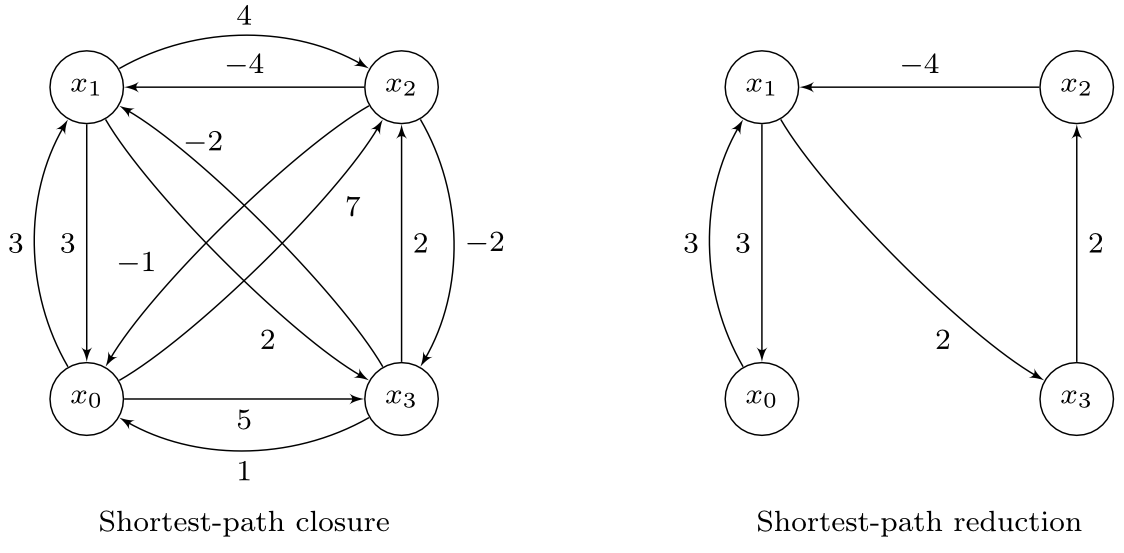
\includegraphics[width=.85\textwidth]{../img/shortest_path.png}
\end{frame}
}

% just for long?
\subsection{Extensions}
\begin{frame}
  \tableofcontents[currentsection, currentsubsection]
\end{frame}

\begin{frame}
  \small
  Decidable extensions:
  \begin{itemize}
    \item \emph{diagonal constraints}: $x - y \odot k$
    \item \emph{updatable} TA: clocks can be reset to any natural number ($x := k \in \mathbb{Z}$) or can be synchronized with another clock ($x := y$)
    \item \emph{urgency} constraints: some locations must be left immediately
  \end{itemize}
  \vfill
  Undecidable extensions:
  \begin{itemize}
    \item \emph{linear} constraints: $\lambda x + \mu y \leq k$
    \item updates such as $x := x + k$ or $x :> k$ (non-determinism)
    \item \emph{stopwatch} automata
    \item \emph{hybrid} automata
    \only<1>{\item ...}\only<2>{\item pretty much everything else you can think of}

  \end{itemize}
\end{frame}

\section{Model Checking Real-Time Systems}
\subsection{Timed Temporal Logic}

\begin{frame}
  \tableofcontents[currentsection, currentsubsection]
\end{frame}

\justfor{short}{
\begin{frame}
  \small
  \begin{definition}[Metric Temporal Logic]
    Given a set of atomic propositions $P$, the formulas of MTL are defined for any time interval $I$ with the \emph{time-constrained until} operator $\text{\bf U}_I$ as follows:
    \begin{equation*}
      \varphi ::= p \in P\ |\ \neg \varphi\ |\ \varphi \land \varphi\ |\ \varphi \text{\bf U}_I \varphi
    \end{equation*}
  \end{definition}
  \vfill
  The \emph{constrained always} $\square_I$ and \emph{constrained eventually} $\lozenge_I$ operators can be defined with $\text{\bf U}_I$ in a similar way as in LTL.
  \vfill
  \onslide<2->{
    \centering
    \Large
    \color{red}
    \fbox{What is $\text{\bf U}_I$?!}
    \onslide<3->{
      \color{black}
      $\rightarrow$ give its semantics
    }
  }
\end{frame}
}
\justfor{long}{
\begin{frame}
  \small
  \begin{definition}[Metric Temporal Logic]
    Given a set of atomic propositions $P$, the formulas of MTL are defined for any time interval $I$ with the \emph{time-constrained until} operator $\text{\bf U}_I$ as follows:
    \begin{equation*}
      \varphi ::= p \in P\ |\ \neg \varphi\ |\ \varphi \land \varphi\ |\ \varphi \text{\bf U}_I \varphi
    \end{equation*}
  \end{definition}
  \vfill
  The \emph{constrained always} $\square_I$ and \emph{constrained eventually} $\lozenge_I$ operators can be defined with $\text{\bf U}_I$ in a similar way as in LTL, namely:
  \begin{align*}
    \lozenge_I \varphi &\triangleq \top \text{\bf U}_I \varphi\\
    \square_I \varphi &\triangleq \neg \lozenge_I \neg \varphi
  \end{align*}
  \vfill
  \onslide<2->{
    \centering
    \Large
    \color{red}
    \fbox{What is $\text{\bf U}_I$?!}
    \onslide<3->{
      \color{black}
      $\rightarrow$ give its semantics
    }
  }
\end{frame}
}

\begin{frame}
\textbf{Continuous semantics}:
$$f \models \varphi_1 \text{\bf U}_I \varphi_2 \quad \text{iff} \quad \exists t \in I, f^t \models \varphi_2 \land \forall u \in (0, t), f^u \models \varphi_1$$
\onslide<2->{
\centering
\begin{tikzpicture}
  \node[label=below:$time$] at (8, 0) {};
  \draw[-] (0,0) -- (1,0);
  \draw (1, 0) [|-|]        -- (6, 0) node[below=10pt, midway] {$I$};
  \draw[->] (6,0) -- (8,0);
  \draw (5,2.8pt) -- (5,-2.8pt) node[below, midway] {$t$};
  {
  \color{blue}
  \draw[decorate,decoration={brace,amplitude=5pt}] (1,0.45) -- (5,0.45)
    node[anchor=south,midway,above=4pt] {$\varphi_1$ is satisfied};
  }
  {
  \color{red}
  \draw[<-, thick] (5,2.8pt) -- (6, 1) node[pos=1,above] {$\varphi_2$ is satisfied};
  }
\end{tikzpicture}
}
\end{frame}

\begin{frame}
\textbf{Pointwise semantics}:
Let $w = ((a_i, t_i))_{i \in \mathbb{N}}$ be a timed word over $2^P$.
\begin{equation*}
  w, i \models \varphi_1 \text{\bf U}_I \varphi_2 \quad \text{iff} \quad
  \exists\ i < j < |w|,
  \begin{cases}
    w, j \models \varphi_2\ &\land \\
    t_j - t_i \in I\ &\land \\
    \forall\ i < k < j,\ w, k \models \varphi_1
  \end{cases}
\end{equation*}
\onslide<2->{
\centering
\begin{tikzpicture}
  \small
  \draw (0,0) -- (0,.5) node [left=1pt, midway] {$w$} -- (8,.5) -- (8,0) -- (0,0);
  \draw (2,0) -- (2,.5) node [right=1pt, midway] {$i$} node [below right, pos=0] {$t_i$};
  \draw (2.5,0) -- (2.5,.5);
  \draw (6,0) -- (6,.5) node [right=1pt, midway] {$j$} node [below right, pos=0] {$t_j$};
  \draw (6.5,0) -- (6.5,.5);
  {
  \color{blue}
  \draw[decorate,decoration={brace,amplitude=5pt}] (2.5,0.55) -- (6,0.55)
    node[anchor=south,midway,above=4pt] {$\varphi_1$ is satisfied};
  }
  {
  \color{green!60!black}
  \draw[decorate,decoration={brace,amplitude=5pt}] (6.5,-0.55) -- (2,-0.55)
    node[anchor=north,midway,below=4pt] {$\Delta t \in I$};
  }
  {
    \color{red}
    \draw[<-, thick] (6.25,.5) -- (6.25, 1.1) node[pos=1, above] {$\varphi_2$ is satisfied};
    }
\end{tikzpicture}

}
\end{frame}


\subsection{Some results}

\begin{frame}
  \tableofcontents[currentsection, currentsubsection]
\end{frame}

\justfor{short}{
\begin{frame}
  \small
  \begin{itemize}
    \item<1-> Reachability and language emptiness for TA are PSPACE-complete
    \vfill
    \item<2-> MC and SAT for LTL are PSPACE-complete over both semantics
    \vfill
    \item<3-> MC and SAT for MTL in the pointwise semantics are decidable over finite words only, and are undecidable in the continuous semantics

    $\rightarrow$ In some subsets of MTL, we can recover decidability
    \vfill
    \item<4-> MC is PSPACE-complete and SAT is undecidable for TCTL
  \end{itemize}
\end{frame}
}
\justfor{long}{
\begin{frame}
  \verysmall
  \begin{itemize}
    \item Reachability and language emptiness for TA are PSPACE-complete

    {\color{blue}Universality, inclusion and equivalence are all undecidable.
    The RA has exponentially larger size, but checking a reachability property can be done on the fly, hence this can be done in polynomial space.}
    \item MC and SAT for LTL are PSPACE-complete over both semantics

    {\color{blue}The PSPACE upper bound can be established by translating the negated formula to a Büchi automaton, and performing an on-the-fly reachability check on the product of this automaton with the region graph of the model.}
    \item MC and SAT for MTL in the pointwise semantics are decidable over finite words only, and are undecidable in the continuous semantics

    {\color{blue}Decidability results are essentially obtained by translating MTL formulas into one-clock alternating timed automata, and rephrasing the model-checking or satisfiability problems as instances of language emptiness in one-clock alternating timed automata.
    Continuous semantics is strictly more expressive!}

    \begin{itemize}
      \verysmall
      \item MC and SAT for MTL over bounded time and MITL are EXPSPACE-complete for both semantics (over finite and infinite words)
      \item MC and SAT for ECTL are PSPACE-complete for both semantics
    \end{itemize}
    \item MC is PSPACE-complete and SAT is undecidable for TCTL
    
    {\color{blue}The idea is to associate universal path-quantifiers with each temporal modality.}
  \end{itemize}
\end{frame}
}

\subsection{Timed Games}
\begin{frame}
  \tableofcontents[currentsection, currentsubsection]
\end{frame}
\justfor{long}{
\begin{frame}
  \small
  \begin{definition}
    A \emph{timed game} is basically a deterministic TA $A_G = (L, \ell_0, C, \Sigma_c \cup \Sigma_u, I, E)$ where $\Sigma_c$ and $\Sigma_u$ are disjoint.
  \end{definition}
  \vfill
  A \emph{strategy} over $[\![A_G]\!]$ is a mapping from finite runs to $\Sigma_c \cup \{\delta\}$.
  \vfill
  The outcome of a strategy is \emph{maximal} either if it stops in a target location or or if no controllable actions are available at its end.
  \vfill
  A strategy is \emph{winning for the reachability game} if any of its maximal outcome and leads to a target location, and \emph{winning for the safety game} if none of its outcomes is accepting.
\end{frame}
}

\begin{frame}
\small
Timed games by example:
\begin{center}
  \begin{figure}
    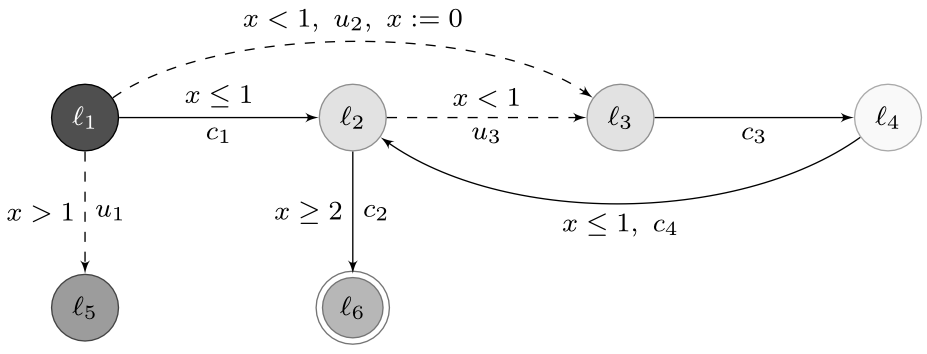
\includegraphics[width=.85\textwidth]{../img/game.png}
    \\
    \tiny{Figure taken from \cite{handbook}}
  \end{figure}
  \begin{tabular}{|ccc|ccc|}
    \hline
    $(\ell_1, v)$ & $\rightarrow$ &
    $\begin{cases}
      \delta \ \text{if}\ v(x) \leq 1\\
      c_1 \ \text{if}\ v(x) = 1
    \end{cases}$ &
    $(\ell_2, v)$ & $\rightarrow$ &
    $\begin{cases}
      \delta \ \text{if}\ v(x) \leq 2\\
      c_2 \ \text{if}\ v(x) \geq 2
    \end{cases}$ \\
    \hline
    $(\ell_3, v)$ & $\rightarrow$ &
    $\begin{cases}
      \delta \ \text{if}\ v(x) < 1\\
      c_3 \ \text{if}\ v(x) \geq 1
    \end{cases}$ &
    $(\ell_4, v)$ & $\rightarrow$ &
    $\begin{cases}
      \delta \ \text{if}\ v(x) \neq 1\\
      c_4 \ \text{if}\ v(x) = 1
    \end{cases}$ \\
    \hline
  \end{tabular}
\end{center}
\end{frame}

\justfor{short}{
\begin{frame}
\small
Remarks:
\begin{itemize}
  \item  The (time-optimal) reachability and safety games are decidable for timed games. They are EXPTIME-complete.

  \item Restriction to non-Zeno is still EXPTIME-complete.
  
  \item TG can be used to check time bisimilarity
\end{itemize}
\end{frame}
}

\justfor{long}{
\begin{frame}
\small
Remarks:
\begin{itemize}
  \item  The (time-optimal) reachability and safety games are decidable for timed games. They are EXPTIME-complete.

  {\color{blue}For reachability as well as safety games, it is sufficient to consider memoryless strategies! Exponential time essentially comes from the region abstraction.}

  \item Restriction to non-Zeno is still EXPTIME-complete.
  
  \item TG can be used to check time bisimilarity in a TA with a simple construction
\end{itemize}
\end{frame}
}

\justfor{long}{
\section{Ongoing challenges}
\begin{frame}
  \frametitle{Ongoing challenges}
  \begin{itemize}
    \item Robustness and implementability: reconcile the semantics of TA with the models they represent
    \item Statistical model checking: stocastic TA
    \item Timed Games: extensions, e.g. where the players have their own objectives
  \end{itemize}
\end{frame}
}

\nocite{AlurDill}
\section{References}
\begin{frame}{References}
  \setbeamertemplate{bibliography item}{\insertbiblabel}
  \bibliographystyle{abbrv}
  \bibliography{../abstract/ref}
\end{frame}

\end{document}